\documentclass{beamer}

\usepackage{multirow}
\usepackage{graphicx}
\usepackage[latin1]{inputenc}
\usepackage[T1]{fontenc}
\usepackage[english]{babel}
\usepackage{listings}
\usepackage{xcolor}
\usepackage{eso-pic}
\usepackage{mathrsfs}
\usepackage{url}
\usepackage{amssymb}
\usepackage{amsmath}
\usepackage{multirow}
\usepackage{hyperref}
\usepackage{booktabs}
\usepackage{bbm}
\usepackage{cooltooltips}
\usepackage{colordef}
\usepackage{beamerdefs}
\usepackage{lvblisting}

\pgfdeclareimage[height=3.5cm]{logobig}{hucaselogo}
\pgfdeclareimage[height=0.7cm]{logosmall}{Figures/LOB_Logo}

\renewcommand{\titlescale}{1.0}
\renewcommand{\titlescale}{1.0}
\renewcommand{\leftcol}{0.6}

\title[Fama French Replication]{Replication of the Fama French 3 Factor Model and Relevance Today}
\authora{Xin Tan }
\authorb{Daria Skidnova}
\authorc{Jeff Giddens}

\def\linka{http://lvb.wiwi.hu-berlin.de}
\def\linkb{http://case.hu-berlin.de}
\def\linkc{}

\institute{Ladislaus von Bortkiewicz Chair of Statistics \\
C.A.S.E. -- Center for Applied Statistics\\
and Economics\\
Humboldt--Universit{\"a}t zu Berlin \\}
\date{June 26th, 2018}
\hypersetup{pdfpagemode=FullScreen}

\begin{document}


\frame[plain]{

\titlepage
}
\section{Introduction}
\begin{frame}[allowframebreaks]

\label{contents}
\frametitle{Structure}

\tableofcontents[sections={1-3}]%[hideallsubsections]
%figure out why they're not numbered
\framebreak
\tableofcontents[sections={4-5}]

\end{frame}

\begin{frame}
\frametitle{Purpose of the Study}

\begin{itemize}
\item replicate the Fama-French Three-Factor model (1993)
\item apply it to recent data (2010-2017)
\item assess the explanatory power for the Fama-French Three-Factor model over different periods

\end{itemize}

\end{frame}

\section{Theory and Design}

\begin{frame}
\frametitle{Theory and Design}
The Capital Asset Pricing Model: 

$$R_i-R_F = \beta_M\cdot(R_M-R_F)$$
%This model, developed in the 1960s, was the only asset pricing model

The Fama-French asset pricing Model: 
$$R_i-R_F = \beta_M\cdot(R_M-R_F) + \beta_S\cdot SMB + \beta_V\cdot HML$$


\begin{itemize}

\item $R_I-R_F$ is an excess return of the stock or portfolio
\item $\beta_M$ is the sensitivity coefficient
\item SMB is a small minus big (in terms of capitalization)
\item HML is high minus low (in terms of book-to-value ratio)

\end{itemize}
\end{frame}


\begin{frame}
\frametitle{Data Preparation for Model Replication}
Data:
\begin{itemize}
\item Fama/French 3 Factors (monthly)	
\item 25 Portfolios Formed on Size and Book-to-Market (5x5) (Value-Weighted)
% The whole dataset is from 1926.07 to 2018.03 corresponding to the Fama and French (1993) 3-factor setup
\end{itemize}


source: Fama French Homepage

\end{frame}

\begin{frame}
\frametitle{Fama/French 3 Factors}
\begin{table}
\begin{tabular}{ | l | c | c | c | c | }
\hline
 & Mkt-RF & SMB & HML & RF \\ \hline
192607 & 2.96 & -2.30 & -2.87 & 0.22\\ \hline
192608 & 2.64 & -1.40 & 4.19 & 0.25\\ \hline
... & & & & \\ \hline
199112 & 10.84 & -2.22 & -4.01 & 0.38\\ \hline
\end{tabular}
\end{table}
\begin{itemize}
\item CRSP firms listed on the NYSE, AMEX, and NASDAQ
\end{itemize}
\begin{align*}
SMB = &\dfrac{1}{3} (Small Value + Small Neutral + Small Growth) -\\
&\dfrac{1}{3} (Big Value + Big Neutral + Big Growth)\\
HML = &\dfrac{1}{2} (Small Value + Big Value) - \dfrac{1}{2}(Small Growth + Big Growth)\\
\end{align*}

%Orally explain SMB and HML
% Where SMB (Small minus Big) is the average return on the three small portfolios minus the average return on the three big portfolios; HML is the average return on the two value portfolios minus the average return on the two growth portfolios; Mkt-RF is the excess return on the market shows the difference between market return and free-risk rate. The first component is value-weight return of all CRSP companies within NYSE, AMEX, or NASDAQ indices.

% 3 groups for value because bigger effect on the market than market cap
\end{frame}

\begin{frame}
\frametitle{25 Value-Weighted Portfolios}
\begin{table}
\centering
\resizebox{\textwidth}{!}
{\begin{tabular}{ | c | c | c | c | c | c | }
\hline
 & Low & 2 & 3 & 4 & High \\ \hline
Small & SMALL LoBM & ME1 BM2 & ME1 BM3 & ME1 BM4 & SMALL HiBM\\ \hline
2 & ME2 BM1 & ME2 BM2 & ME2 BM3 & ME2 BM4 & ME2 BM5\\ \hline
3 & ME3 BM1 & ME3 BM2 & ME3 BM3 & ME3 BM4 & ME3 BM5\\ \hline
4 & ME4 BM1 & ME4 BM2 & ME4 BM3 & ME4 BM4 & ME4 BM5\\ \hline
Big & BIG LoBM & ME5 BM2 & ME5 BM3 & ME5 BM4 & BIG HiBM\\ \hline
\end{tabular}}
\caption{Structure of the 25 Value-Weighted Portfolios}
\end{table}% explain low and high Book to market (high is value stock, low is growth stock)
\begin{itemize}
\item High BM (Book to Market) stocks are value stocks
\item Big ME (Market Equity) stocks are large companies by market capitalization
\item Each value is that portfolio's monthly percentage return 
\item 
%before subtracting the risk free rate 

%\item The 25 portfolios are formed each year (during year stocks can drop out but not enter) by dividing stocks into 5 groups of Market Eauity and 5 groups of Book to Market Value
% how it's calculated: 
%ME is determined 
%Book to market determined in december of the previous year (6-17 months prior to the current month)
% 3 for value because has larger effect than firm size

\end{itemize}


\end{frame}


\subsection{The Fama-French Three-Factor Model}
%explain the data and the backgroud  

\subsection{Data Preparation}
%data description 3 things -  fdjksaldg
% 2 datasets - fama french data and SP500 data
% how we treat NA is differeing in 2010-2017, why we cut in 5 year blocks 

%1. prepare for replication model, how to download data, deal with data (in 25 portfolio several ways to cut the data - equal weighted/valued weighted - choose value weighted) explain the 2x3 regressor porfolio creation 
% explain both
% data cleaning and transforming: 
% NA, and on average 251 trading days and some stocks have missing data for one day, so they are all discounted, but fortunately approximately 481 (tk) out of the 500 are counted)
%running the data takes an hour, so all was stored as csv files

\begin{frame}
\tableofcontents[currentsection,hideothersubsections]

\end{frame}



\section{Replicating the Three-Factor Model}
%


\label{current spot}


\begin{frame}
\tableofcontents[currentsection,hideothersubsections]

\end{frame}


\subsection{Batch Regression}
\begin{frame}[fragile]
\frametitle{Batch Regression}
\begin{itemize}
\item Use multivariate regression
\end{itemize}
\begin{lstlisting}
# batch regressing 25 portfolios 
results <- list()
# Data starts from the 2nd col of P25
for (i in 1:(ncol(P25) - 1)) { 
  rirf <- unlist (P25[, i + 1]) - rf   
     y <- lm (rirf ~ rmrf + smb + hml)
  results[[i]] <- summary (y)
}
\end{lstlisting}
\end{frame}
% 1. bring in the two tables
% 2. separate the relevant columns
% 3. open an empty list called results to fill with summary statistics of the batch regression
% 4. Regression is run on each portfolio results are saved in a list


\subsection{Formatting the Results}
\begin{frame}[fragile]
\frametitle{Formatting the Results}
\begin{itemize}
\item Save all coefficients of regression results as vectors
\end{itemize}
\begin{lstlisting}
for(i in 1:(ncol(P25)-1)) {
  betas <- cbind(betas,results[[i]]$coefficients[,1])
  std.errors <- cbind(std.errors,results[[i]]$sigma)
  t.values <- cbind(t.values, results[[i]]$coefficients[,3])
  R.squareds <- cbind(R.squareds, results[[i]]$adj.r.squared)
}

\end{lstlisting}
\end{frame}
% bullet is the part of code not shown 
% the -1 is to remove the date column
% now each of these objects is a table 
\begin{frame}[fragile]
\frametitle{Replicating Table 6 (1993)}
\begin{itemize}
\item Resize the output to 5x5 format as in the Fama-French paper
\end{itemize}
\begin{lstlisting}
resize <- function(x) {
  df = data.frame (matrix(x, nrow=5, byrow = TRUE))
  colnames(df) = c("Low", "2", "3", "4", "High")
  rownames(df) = c("Small", "2", "3", "4", "Big")
  return(df)
}

\end{lstlisting}
\end{frame}

\subsection{Comparison with the Original Fama-French Results}
\begin{frame}
\begin{figure}
\centering
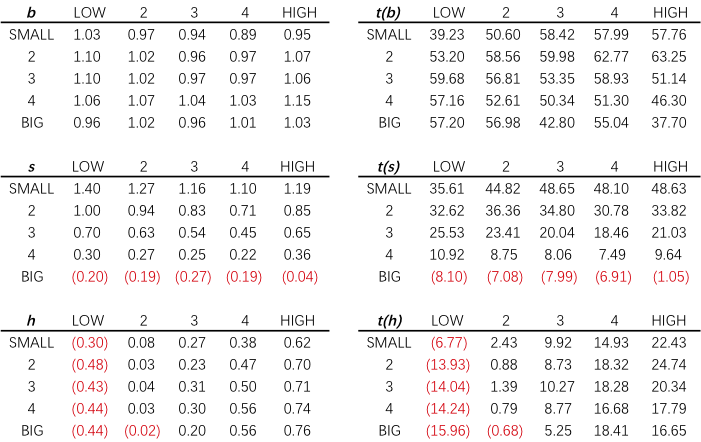
\includegraphics[scale=.8]{FF3results.png}
\caption{Results of the Fama French 3 Factor Model}
\end{figure}
\end{frame}


\begin{frame}
\begin{figure}
\centering
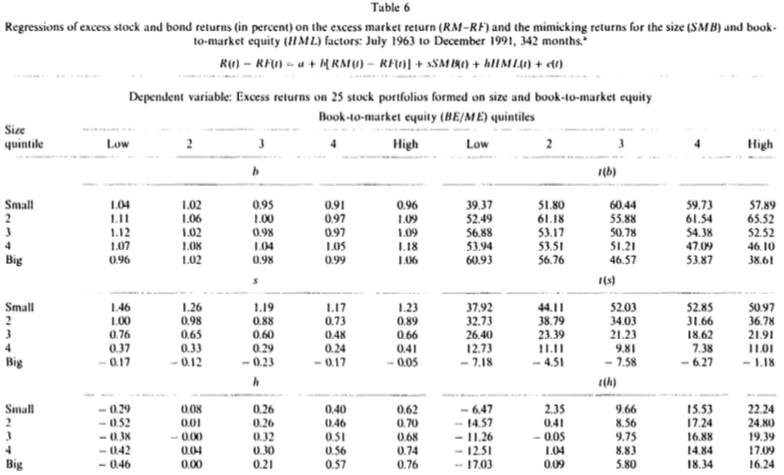
\includegraphics[scale=.35]{FF1993-Table6.png}
\caption{Results of the Fama French 3 Factor Model in Fama and French 1993b}
\end{figure}
\end{frame}

\section{Applying the Fama-French Model to the S\&P 500}

\begin{frame}
\tableofcontents[currentsection,hideothersubsections]

\end{frame}

\subsection{Data Preparation}

\begin{frame}[fragile]
\frametitle{Retrieving S\&P 500 Data}
Download the S\&P 500 stocks from Yahoo finance

\end{frame}

\begin{frame}[fragile]
\frametitle{Retrieving S&P500 Data}
\begin{itemize}
\item Download S\&P 500 adjusted stock prices
\end{itemize}
\begin{lstlisting}
stocks<-BatchGetSymbols(tickers = companies$tickers, 
                 first.date = "2010-01-01",
                 ast.date = "2017-12-31")

# Select the good tickers
good.tickers <- stocks$df.control$ticker [stocks$df.control$threshold.decision == "KEEP"]
\end{lstlisting}
\begin{itemize}
\item stocks is a list that contains 2 dataframes:
\begin{itemize}
\item df.control contains descriptive information %like whether the download for the ticker is successful.
\item df.tickers contains the downloaded price data %Each row is the price data for one ticker at one date, hence we need to process the data into a format easier to work with.
\end{itemize}
\end{itemize}
\end{frame}
%/ 465 stocks are "KEEP" for 2010 - 2017

\begin{frame}[fragile]
\frametitle{Creating a data frame of S\&P 500 Prices}
\begin{itemize}
\item Use the dates of 3M as the date column of the data frame
\item Merge price data of stocks into the data frame %matching the dates
\end{itemize}
\begin{lstlisting}
SP500.data <- data.frame(date = stocks$df.tickers[stocks$df.tickers$ticker == "MMM", "ref.date"])

for(i in 1:length(good.tickers)){ 
    X <- data.frame(
    stocks$df.tickers[stocks$df.tickers$ticker == good.tickers[i], c("ref.date", "price.adjusted")])
    colnames(X) <- c("date", as.character(good.tickers[i]))
    SP500.data <- merge.data.frame(SP500.data, X, by = "date", all.x = TRUE)
}
\end{lstlisting}

\end{frame}
%create the table similar to teh big 25 column table, except 500 column table
%write table at end - SP500 data
%steps:
%1. Create 1 column date table based on MMM ticker (because always traded)
% Use the dates from MMM data as the date column for the data frame SP500.data
%2. merge 500 individual stocks into data frame, matching to dates
%3. 

\begin{frame}[fragile]
\frametitle{Convert daily data to monthly return}
\begin{itemize}
\item Convert downloaded daily data to monthly price data series into XTS series
\item quantmod::monthlyReturn()requires non-NA daily prices in xts format
\end{itemize}
\begin{lstlisting}
Stock.Prices.Daily <- xts(Stock.Prices.Daily[,-1], order.by = as.POSIXct(Stock.Prices.Daily$date))

Stock.Prices.Daily <- Stock.Prices.Daily[!is.na(Stock.Prices.Daily)]

Stock.Prices.Monthly <- monthlyReturn(Stock.Prices.Daily)
\end{lstlisting}

\end{frame}

\begin{frame}
\frametitle{Data Cleaning}
\begin{itemize}
\item \textbf{Removing stocks with NAs} in the series ensures that remaining stocks have same number of observations
\item \textbf{Remove NAs in each series} results in a smaller sample size 
\end{itemize}

Price data with NAs in the middle would result in inaccurate monthly returns. 

\begin{tiny}(BHY Brighthouse Financial Inc. removed for 2015-2017 runs)
\end{tiny}

%We need to remove NAs for using the monthlyReturn() function. Most NAs are due to data not available on the starting date of the series, e.g. the company has not IPO yet. 
Here we face choices: 
\begin{enumerate}
\item Remove all columns with NAs, then all remaining stocks could have the regression in the same period, i.e. with the same number of observations. (2010-2017) 

\item Dynamically frame the data based on the available non-NA data points, but then some stocks in the regression analysis will have fewer observations. (1980-2015 every 5 years case) 
\end{enumerate}

\end{frame}

\subsection{Fama-French in 2010-2017}
\begin{frame}[fragile]
\frametitle{FamaFrench in 2010-2017}
\begin{lstlisting}
SP500.data <- read.csv("Data/SP500_price.adjusted_2010-2017.csv")
SP500.data$date <- as.Date(SP500.data$date)

# ...

Results <- list()
for(i in 1:ncol(Stock.Prices.Monthly)) {
  RiRF <- Stock.Prices.Monthly[,i] - FF$RF
  Regression <- lm(RiRF ~ FF$Mkt.RF + FF$SMB + FF$HML)
  Results[[i]] <- summary(Regression)
}
\end{lstlisting}
\end{frame}

\begin{frame}
\frametitle{Boxplot of the regression results}

\begin{figure}
\centering
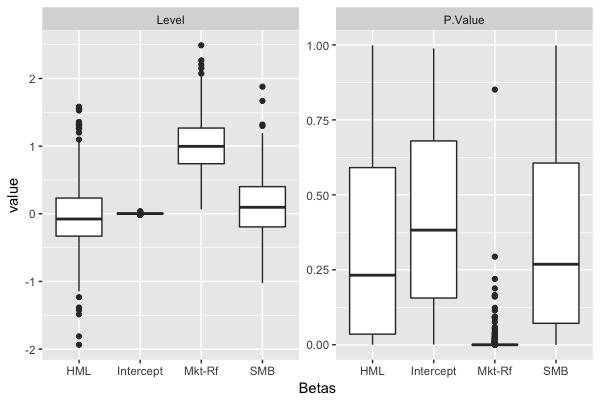
\includegraphics[scale=.4]{1FF3Betas.png}
\end{figure}


\end{frame}

\begin{frame}[fragile]
\frametitle{Goodness of Fit}
\begin{figure}
\centering
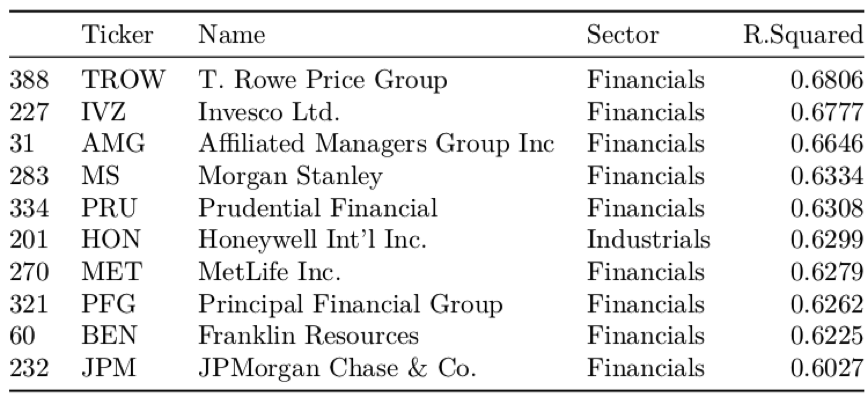
\includegraphics[scale=.5]{goodnessoffittable.png}%This table is out of date
\caption{This table needs to be updated! }%change later
\end{figure}

\end{frame}

\subsection{Trend Analysis in 1980-2015}
\begin{frame}[fragile]
\frametitle{Trend analysis in 1980-2015}
\begin{itemize}
\item loop over above codes to download data from 1980 - 2015, group every 5 years
\end{itemize}
\begin{lstlisting}
library(lubridate)
List.of.start.date <- seq(as.Date("1980/1/1"), as.Date("2016/1/1"), "years")
List.of.start.date <- List.of.start.date[year(List.of.start.date)%%5==0]
\end{lstlisting}
%not shown on slide:
%Download.Stat <- data.frame(Data = List.of.start.date)
%temp <- vector()

%for(i in 1:(length(List.of.start.date)-1))
%{
 % start.date <- as.Date(List.of.start.date[i])
 % end.date <- as.Date(List.of.start.date[i+1])-1
 % #...
 % }

\end{frame}

\begin{frame}
\begin{figure}
\centering
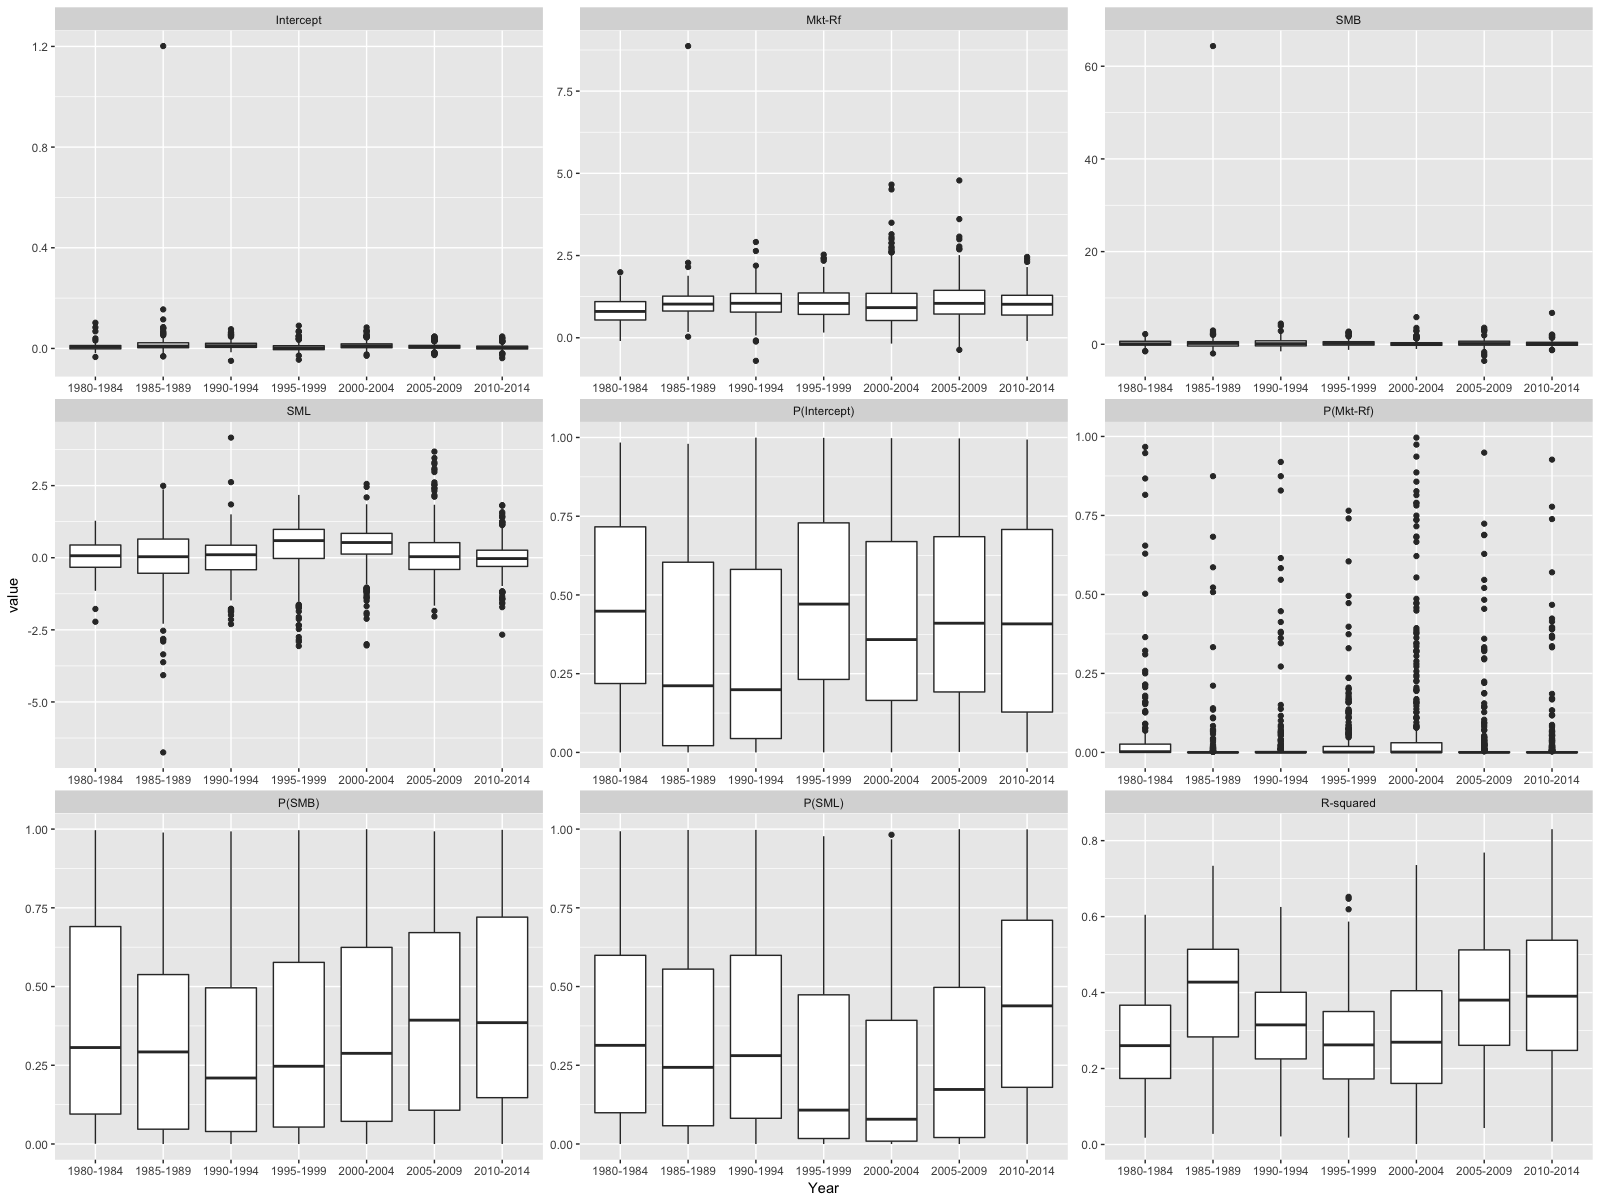
\includegraphics[scale=.16]{2SP500-1980-2015.png}
\caption{Trend analysis in 1980-2015 of full sample}
\end{figure}
\end{frame}
%the scale on upper right box is different due to the outlier

\begin{frame}
\begin{figure}
\centering
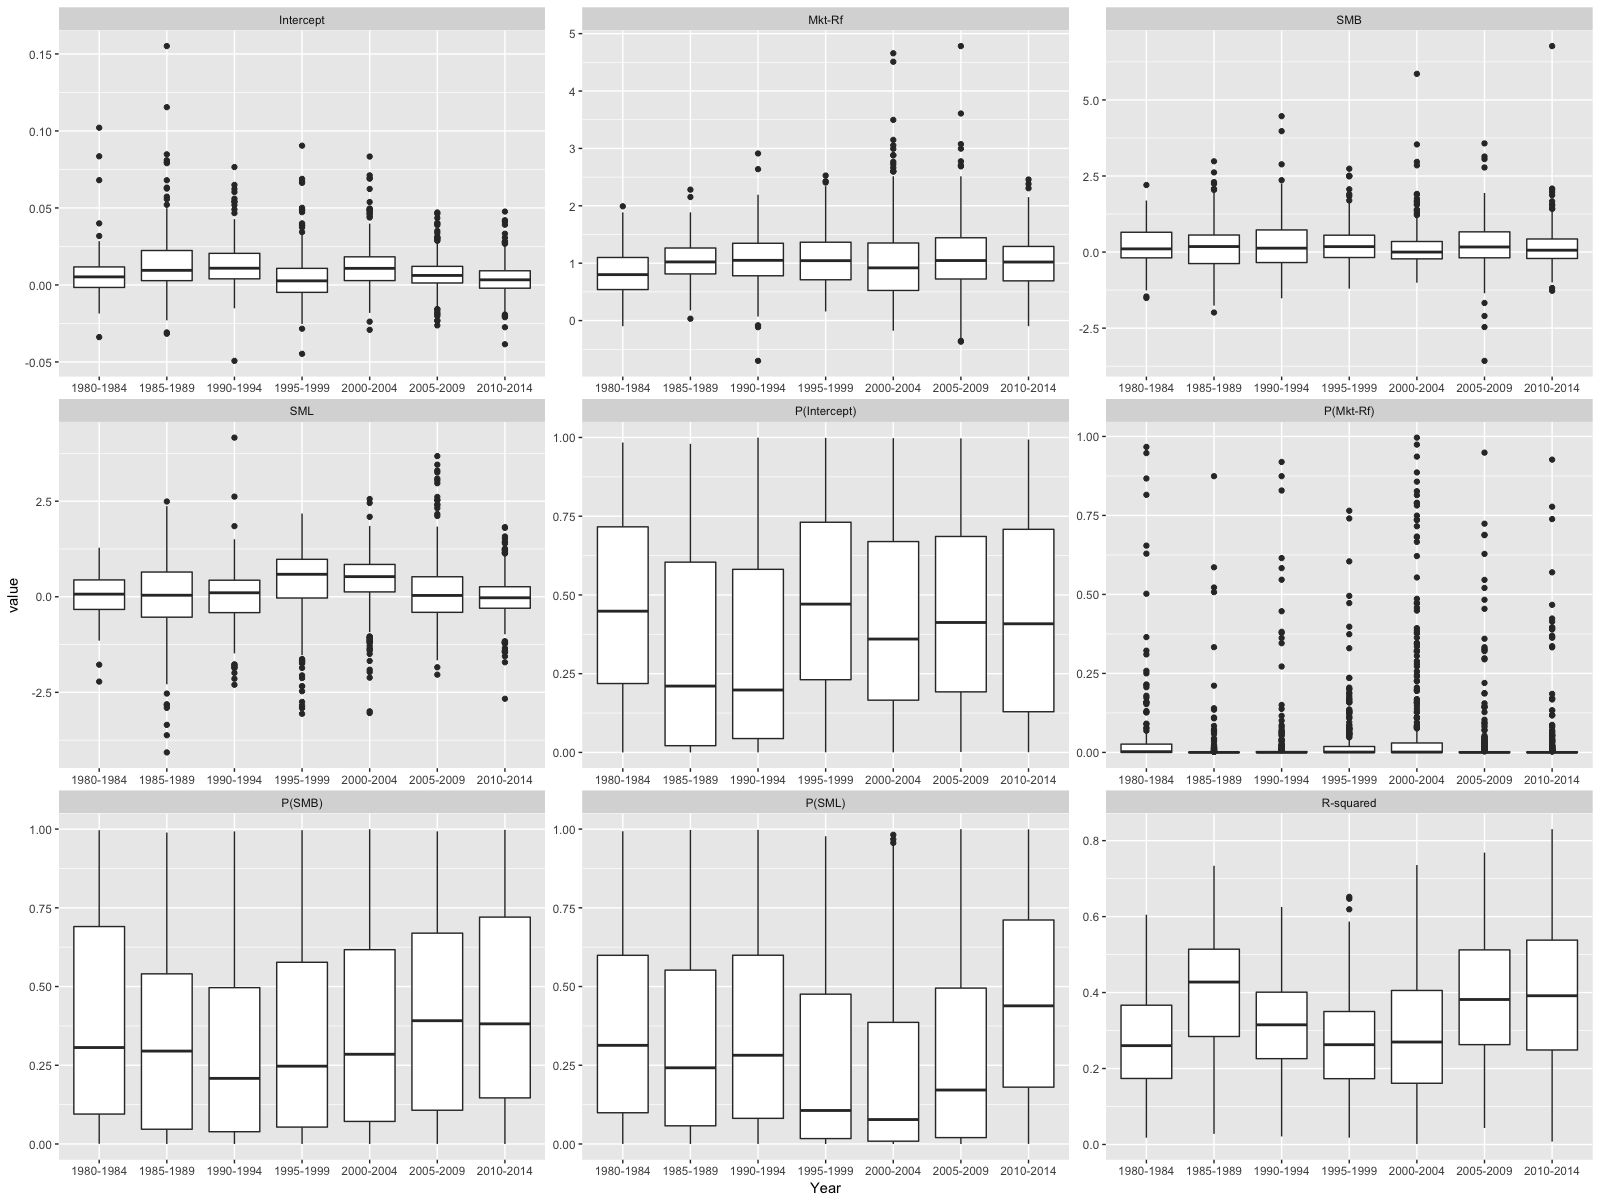
\includegraphics[scale=.16]{3SP500-1980-2015-no-MNST.png}
\caption{Trend analysis in 1980-2015 without MNST}
\end{figure}

\end{frame}

\begin{frame}
\begin{figure}
\centering
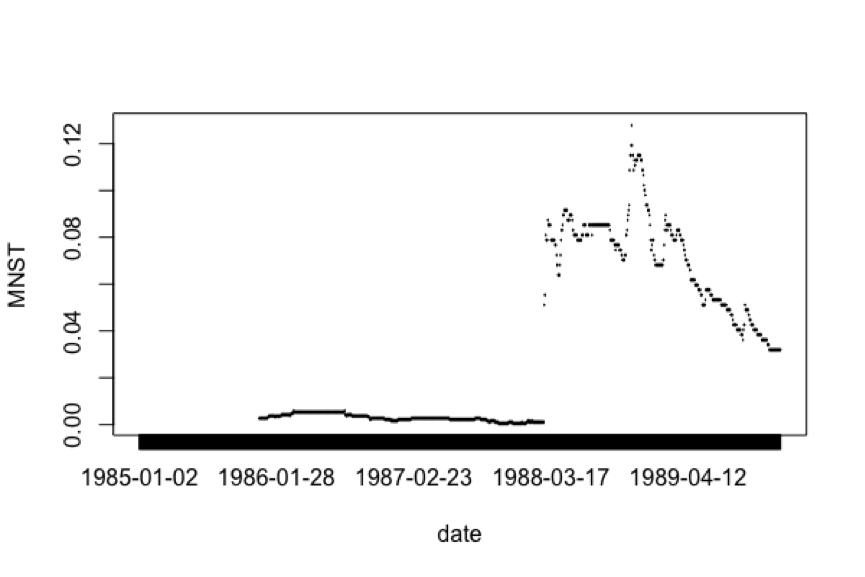
\includegraphics[scale=.6]{weirdgraph.png}
\caption{Monthly Return of MNST (Monster Beverage Corp)}
\end{figure}

\end{frame}

\subsection{Varying Sample Sizes}
\begin{frame}
\frametitle{Varying Samples}
\begin{figure}
\centering
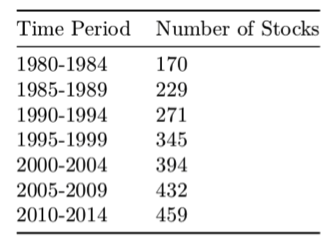
\includegraphics[scale=1.15]{samplestable.png}
\caption{Varying Samples: Sample sizes in each time period}
\end{figure}

\end{frame}

\begin{frame}
\begin{figure}
\centering
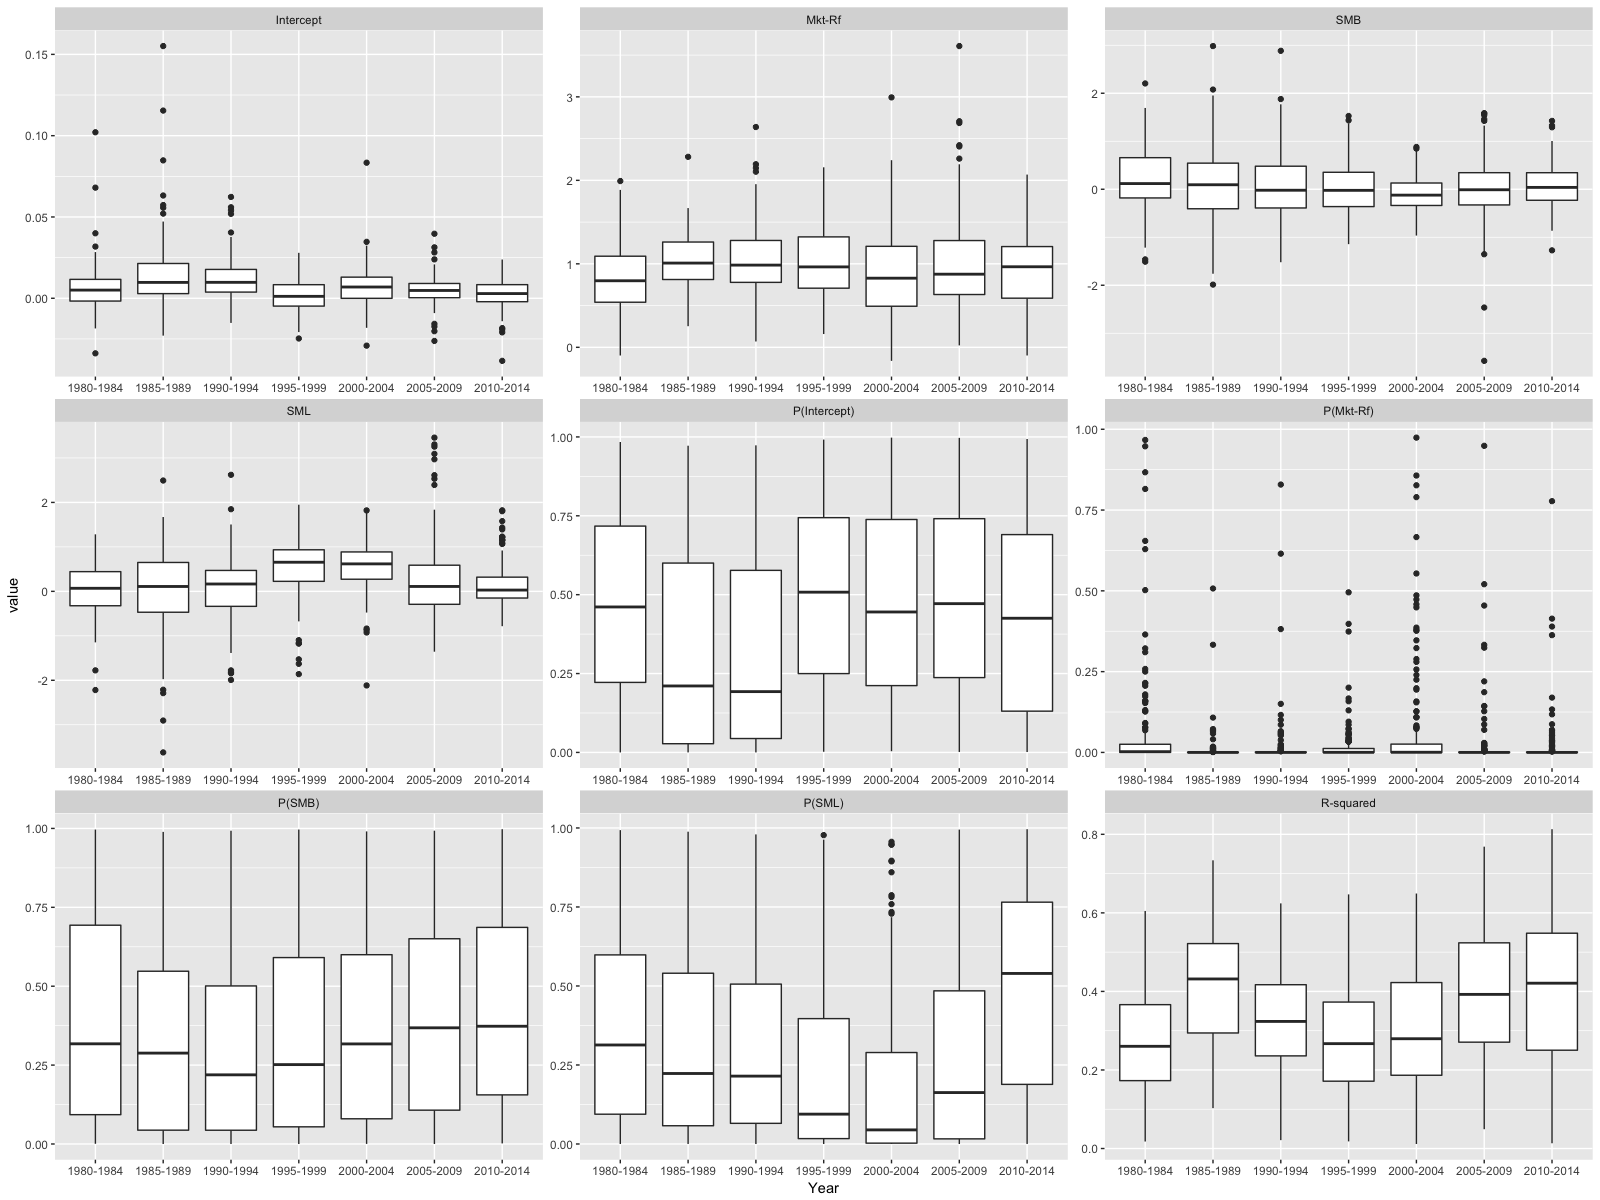
\includegraphics[scale=.16]{3SP500-1980-2015-168-stock.png}
\caption{Trend analysis of 168 stocks listed from 1980-2015}
\end{figure}

\end{frame}

%because we have cut 5 year periods, potentially problematic
% Prove there is no problem, becuase data is drawing from same distribution, so no impact on result 

\begin{frame}
\begin{figure}
\centering
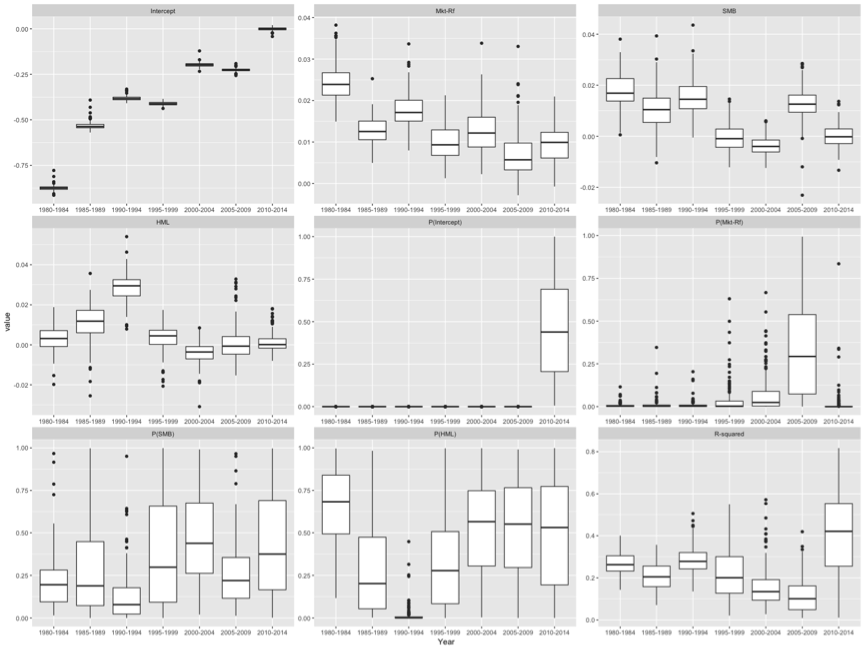
\includegraphics[scale=.6]{samplesplots.png}
\caption{168 Stocks idk what else}
\end{figure}

\end{frame}

\subsection{Correlation of The factors and Top 20 and Bottom 20 returns}
% if you hold from 2010-2017, return over that period, top one netflix 24x
% FOr top 20 highest returning companies, as a portfolio, they are positivitley correlated  with the three factors, exact opposite for bottom 20
% if stocks are high value, return is higher, and smaller company return is higher
\begin{frame}
\frametitle{Correlation of The factors and Top 20 and Bottom 20 returns}

\begin{minipage}{.5\textwidth}
\begin{figure}
\centering
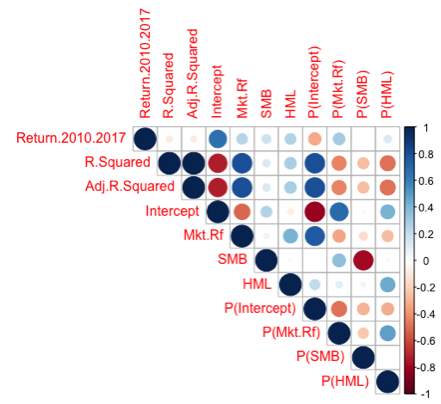
\includegraphics[scale=.66]{correlationfigure1.png}%the sizes are not perfect
\caption{Top 20}
\end{figure}
\end{minipage}%
\begin{minipage}{.5\textwidth}
\begin{figure}
\centering
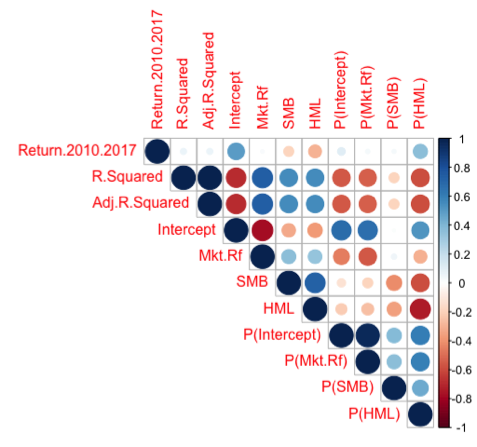
\includegraphics[scale=.6]{correlationfigure2.png}
\caption{Bottom 20}
\end{figure}
\end{minipage}

\end{frame}


\section{Conclusion}
\begin{frame}
\frametitle{Conclusion}



\end{frame}

\end{document}
